\renewcommand{\theauthor}{Matthias Franz}

\chapter{Projektmanagement und Organisation}
In diesem Kapitel geht es um die organisatorischen- und managementbezogenen Teile der Diplomarbeit. Es geht um Scrum und die Anwendung von Scrum innerhalb dieses Projektes und der allgemeinen Abhandlung von Projektmanagement.

\label{sec:ProjUOrg}

\section{Auftraggeber - Intact Systems}
\label{sec:Auftraggeber}
Unsere Diplomarbeit wurde im Auftrag des Unternehmens Intact Systems durchgeführt. Intact Systems ist eine in Lebring sitzende Softwareentwicklungsfirma welche auf Audits, Zertifizierungsmanagement, Rückverfolgbarkeit und Qualitätsmanagement spezialisiert ist und auch Sitze in der USA und in der Schweiz hat. Unsere Ansprechpartner waren Rudolf Rauch und Mathias Schober. Intact bietet maßgeschneiderte und standardisierte Softwarelösungen. Deren bekanntestes Produkt ist Ecert, welches interne Audits, Zertifizierung, Gütesiegel, Lieferanten und noch vieles mehr managen kann.
	\subsection*{Kontaktaufnahme mit Intact Systems}
	Mit Intact Systems wurde am Recruiting-Day der HTBLA Kaindorf Kontakt aufgenommen und Kontaktdaten wurden ausgetauscht. Nach wenigen Emails wurde das erste Treffen vereinbart und die Abhandlung der Diplomarbeit mit Unterstützung von Intact war fixiert. Im gleichen Treffen wurde bereits das Thema der Diplomarbeit im Groben besprochen.  
	
\section{Projektmanagement}
\label{sec:Projektmanagement}
Das Projekt wurde nach der Scrum-Vorgehensweise durchgeführt. Allerdings wurde von der Scrum-Vorgehensweise abgewichen, da manche Eigenschaften für unser Projekt keinen Sinn gemacht hätten, oder gar nicht funktioniert hätten.
	\subsection{Scrum}
	Anstatt ein Projekt am Anfang des Projektes komplett durchzuplanen und langfristige Meilensteine zu setzen, gibt es bei Scrum sogenannte Sprints. Ein Sprint ist ein Zeitintervall unter 4 Wochen, an dessen Beginn ein Ziel für diesen Sprint festgelegt wird, an diesem Ziel wird dann im Sprint gearbeitet. Nach jedem Sprint sollte ein Teil des Projekts fertig werden. Durch diese Herangehensweise baut sich das fertige Projekt mit der Zeit von selbst auf. Wichtig bei Scrum sind Artefakte, Rollen und Meetings.
	\subsubsection{Artefakte}
	\label{sec:Artefakte}
		Artefakte sind Dokumente oder Grafiken welche jeden Projektbeteiligten helfen Übersicht zu behalten. Die wichtigsten Artefakte sind: Vision-Dokument, Product-Backlog, Product-Increment und der Sprint-Backlog.\\
		
			\textbf{Vision-Dokument}\\
				Das Visionsdokument befasst sich im Groben damit, worum es im Projekt geht. Es beschreibt den Zweck und das Ziel oder die Ziele des Projekts. Rahmenbedingungen wie zum Beispiel Budget oder Zeit werden ebenfalls im Visionsdokument festgehalten. Im Visionsdokument wird das geplante Produkt mit ähnlichen bereits existierenden Produkten anderer Unternehmen verglichen und es wird erwägt, welche Vorteile gegenüber den bereits existierenden Produkten existieren.
			Das Wichtigste am Visionsdokument ist, dass das fertige Produkt von Anfang des Projektes an verständlich niedergeschrieben ist, sodass keine Verwirrungen entstehen. \\ 
						
			\textbf{Product-Backlog} \\
				Der Product-Backlog wird vom Product-Owner verfasst und gepflegt. Weitere Funktionen des Product-Owners werden in \ref{sec:Rollen} beschrieben. Der Product-Backlog beinhaltet alle Anforderungen an das Projekt und ist somit für eine erfolgreiche Durchführung des Projekts von hoher Bedeutung. Der Product-Backlog wird nicht einfach einmal am Projektbeginn verfasst und bleibt dann für die Restdauer des Projektes unbearbeitet, sondern wird über die gesamte Projektlaufzeit verändert. Der Product-Owner kann neue Einträge hinzufügen, bereits vorhandene Beiträge bearbeiten oder schlicht und einfach Beiträge entfernen. \\
				Einträge des Product-Backlogs werden Product-Backlog Items genannt, diese Items können folgendes sein: 
				\begin{itemize}
					\item Qualitätsanforderungen
					\item Funktionale Anforderungen
					\item User-Stories
					\item Fehler (Bugs)
					\item Verbesserungen
				\end{itemize}
				Wie diese Product-Backlog Items im Endeffekt niedergeschrieben werden, ist dem Product-Owner überlassen. Jedoch sollte jedes Product-Backlog Item eine Priorität, Aufwandsschätzung und Beschreibung haben.\\ vgl.\textcite{ScrumProduct-Backlog} \\
				Ein Product-Backlog Item kann eine User-Story sein. Diese User-Stories sind der wichtigste und am häufigsten auftretende Inhalt eines Product-Backlogs. User-Stories sind kurze Beschreibungen von Funktionalitäten, welche das Programm haben soll. Diese werden immer aus der Sicht einer Gruppe geschrieben, zum Beispiel: Als Benutzer möchte ich meine Arbeit mit anderen Benutzern teilen. \\
				Es gibt zahlreiche Anwendungen welche es ermöglichen Product-Backlogs zu erstellen. In diesem Projekt wurde Excel verwendet, da es einfach ist und alles bietet was benötigt wird, um einen brauchbaren Product-Backlog zu verfassen. Wie in Abbildung \ref{fig:productBacklog} zu sehen ist, kann man Product-Backlog Items auch nach Kategorien ordnen. \\
\begin{figure}[H]	
	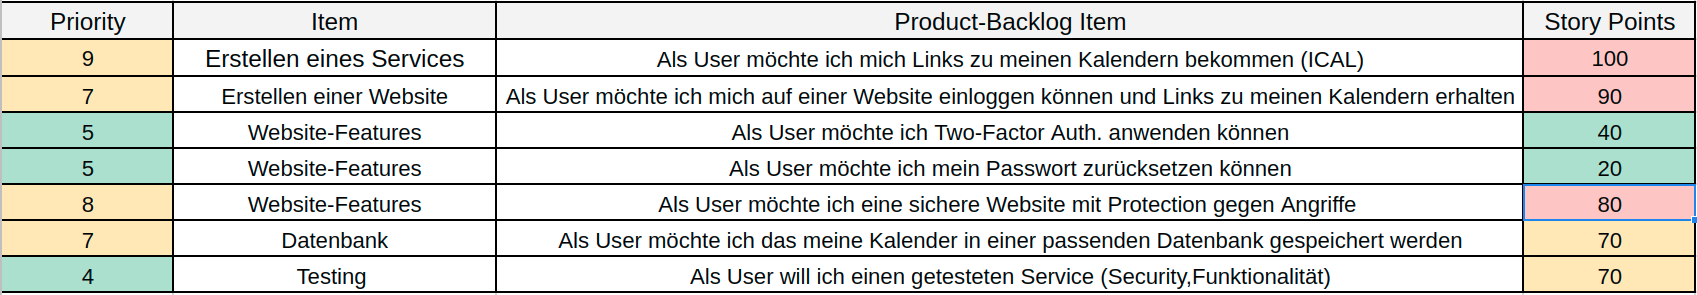
\includegraphics[width=\textwidth]{ProjektmanagementUndOrganisation_ProductBacklog}
    \caption{Product-Backlog}
    \label{fig:productBacklog}
\end{figure}
				
			\textbf{Product-Increment} \\
			Das Ziel von Scrum ist es, nach jedem Sprint ein potenziell veröffentlichbares Produkt vorzeigen zu können. Dieses Produkt muss getestet, fertig und von hoher Qualität sein. Ein Beispiel wäre, dass nach einem Sprint ein Benutzer sich anmelden können soll, bedeutet aber nicht, dass der Benutzer sich auch abmelden können muss. Somit muss nach einem Sprint ein fertiges und funktionierendes Stück Software vorweisbar sein. Das heißt allerdings nicht, dass andere Funktionen, welche mit der Funktion in diesem Sprint implementiert wurden, zusammenhängen auch fertiggestellt werden müssen. Das Product-Increment ist kein Dokument sondern Code welcher nach jedem Sprint fertig und funktionstüchtig sein muss.\\ vgl. \textcite{ScrumProduct-Increment}\\

			\textbf{Sprint-Backlog} \\ 
			Vor jedem Sprint gibt es ein Sprint-Planning Meeting welches in \ref{sec:Rollen} erklärt wird. In diesem Meeting wird der Sprint-Backlog angefertigt. Der Sprint-Backlog beinhaltet Einträge aus dem Product-Backlog welche im kommenden Sprint durchgeführt werden sollen. Der Product-Owner hat das finale Entscheidungsrecht welche Product-Backlog Items letztendlich in den Sprint-Backlog gelangen. Es werden oft auch noch genauere Informationen zu den Elementen aus dem Product-Backlog hinzugefügt falls zusätzliche Informationen benötigt werden.
			Einträge im Sprint-Backlog werden Sprint-Backlog Tasks genannt. Der Aufwand einzelner Sprint-Backlog Tasks wird wie beim Product-Backlog geschätzt und niedergeschrieben.\\
			Wie die Sprint-Backlog Tasks abgearbeitet werden bestimmt das Team welches in \ref{sec:Rollen} beschrieben wird. Das Team hat auch die Aufgabe den Sprint-Backlog zu pflegen, indem der Status von Sprint-Backlog Tasks verändert wird. Wenn ein Eintrag gerade durchgeführt wird, ist er ,,In Arbeit``, fertige Tasks werden mit ,,Fertig`` markiert, und Einträge welche noch nicht in Bearbeitung sind werden mit ,,Offen`` markiert um den Sprint-Backlog übersichtlich zu gestalten. Diese Benennungen sind aber dem Team selbst überlassen, sollten allerdings nicht weggelassen werden.\\ vgl. \textcite{ScrumSprint-Backlog} \\ 
	\subsubsection{Rollen}
	\label{sec:Rollen}
		Bei Scrum wird das Team in Rollen eingeteilt und jede Rolle hat eine spezielle Funktionalität welche im Laufe des Projekts durchgeführt werden muss. Eingeteilt wird in Product Owner, Scrum-Master und das Team. \\

			\textbf{Product Owner} \\
			Der Product Owner oder kurz PO ist essenziell für eine erfolgreiche Durch-\\führung von Scrum. Der PO ist kein Komitee, sondern immer nur eine Person. Auch wenn der PO kein Komitee ist, kann er oder sie ein Komitee vertreten. Der Product-Backlog wird vom PO erstellt und der PO muss sicherstellen, dass das Team jeden Eintrag im Product-Backlog versteht. Genaueres zum Product-Backlog im Kapitel \ref{sec:Artefakte}. Die wichtigste Aufgabe des Product-Owners ist die Verbesserung der Effizienz des Teams. Dies kann erreicht werden indem Product-Backlog Items ordentlich priorisiert werden und der PO mit Stakeholdern kommuniziert und diese über die aktuellen Ergebnisse informiert. Weiters ist der PO für die Leistungskontrolle zuständig. Er oder sie erklärt Product-Backlog Items für fertig oder nicht.\\vgl. \textcite{ScrumProductOwner} \\ 
			
			\textbf{Scrum-Master} \\
			Die Hauptaufgabe des Scrum-Masters ist es, sicherzustellen dass der Scrum-Prozess ordentlich durchgeführt wird. Dies geschieht indem er oder sie Konflikte im Team stillt, einen Blick auf die Artefakte hat und Hindernisse beseitigt welche sich im Entwicklungszyklus ergeben können. Der Scrum-Master ist die Kommunikationsschnittstelle zwischen dem Team und dem Product-Owner welche beide im Kapitel \ref{sec:Rollen} näher behandelt werden. Weiters moderiert ein Scrum-Master Meetings welche im Scrum-Prozess anfallen. Der Scrum-Master ist allerdings nicht der Projektleiter. Er oder sie befasst sich mit dem Scrumablauf und nicht damit wie einzelne Funktionalitäten implementiert werden. Ein Scrum-Master welcher gleichzeitig Teammitglied oder Product-Owner ist, kann zu Interessenskonflikten führen und sollte somit vermieden werden.\\vgl. \textcite{ScrumScrumMaster} \\
			
			\textbf{Team} \\
			In einem Scrum-Prozess gibt es zwei Teams. Das Team im allgemeinen welches aus Product-Owner, Scrum-Master und dem Entwicklungsteam besteht, und das Entwicklungsteam im Einzelnen. Dieses Kapitel wird sich mit dem Entwicklungsteam befassen. Die Aufgabe des Entwicklungsteams ist es, am Ende eines Sprints ein potenziell lieferbares Product-Increment fertiggestellt zu haben. Eine Erklärung zum Product-Increment ist im Kapitel \ref{sec:Artefakte}. Entwicklungsteams sind selbstorganisierend, das heißt, dass niemand dem Entwicklungsteam vorschreiben kann wie sie etwas zu machen haben.\\
			Die Größe des Teams spielt eine wichtige Rolle in der Produktivität. In einem kleinen Team wird es nur selten zu Kommunikationsproblemen kommen aber es ist schwierig mit einem kleinen Team alle Kenntnisse welche für ein Projekt benötigt werden abzudecken. Ein zu großes Team vergrößert den organisatorischen Aufwand enorm und ist somit trotz wahrscheinlicher Abdeckung aller benötigten Kenntnisse nicht in der Lage, wünschenswerte Ergebnisse zu erbringen. Ein Team von 4 - 6 Entwicklern und Entwicklerinnen ist nur selten falsch.\\vgl. \textcite{ScrumTeam} \\
			
		
	\subsubsection{Meetings}
	\label{sec:Meetings}
		Meetings sind ein extrem wichtiger Teil des Scrumprozesses, solange sie gut geleitet und von jedem Teammitglied ernst genommen werden. Nur dann können sie die Effizienz enorm steigern. Essentielle Ereignisse sind das Sprint-Planning Meeting, der Daily-Scrum, die Sprint-Retroperspective und der Sprint-Review.  \\
		
		\textbf{Sprint-Planning Meeting} \\
		Das Sprint-Planning Meeting wird vom Scrum-Master ausgerufen und dauert maximal 8 Stunden für einen einmonatig langen Sprint. Für kürzere Sprints ist das Sprint-Planning Meeting in der Regel kürzer. Das Sprint-Planning-Meeting befasst sich damit, was im bevorstehenden Sprint gemacht wird und wie es ausgeführt wird. Es werden Elemente aus dem Product-Backlog genommen und werden in den Sprint-Backlog verschoben. Beide dieser Artefakte werden im Kapitel \ref{sec:Artefakte} genauer behandelt.\\vgl. \textcite{ScrumSprint-Planning} \\
		
		\textbf{Daily-Scrum} \\
		Wie es der Name bereits sagt, ist der Daily-Scrum ein kurzes tägliches Meeting welches nicht länger als 15 Minuten dauern sollte. Der Daily-Scrum ist ein sogenanntes ,,Standup-Meeting``, dies bedeutet, dass während des Meetings nicht gesessen werden soll. Der Grund dafür ist, dass wenn sich hingesetzt wird alle Beteiligten entspannter sind und desto entspannter die Teilnehmer des Daily-Scrums sind umso länger dauert es. 
		Teilnehmer sind das Team, der Scrum-Master und im gegebenen Falle auch der Product-Owner. Während des Meetings berichtete jedes Entwicklerteammitglied was er oder sie seit dem letzten Daily-Scrum erreicht hat, was er oder sie bis zum nächsten Daily-Scrum vor hat und welche Probleme aufgetreten sind. Die Funktion des Scrum-Masters im Daily-Scrum ist es, das Meeting zu moderieren und sich die Probleme der Entwicklungsteammitglieder aufzuschreiben.
		Das Ziel des Daily-Scrum ist es, alle Beteiligten auf den gleichen Stand zu bringen.\\vgl. \textcite{ScrumDailyScrum} \\
		
		\textbf{Sprint-Retroperspective} \\
		Ein Merkmal von Scrum ist die kontinuierliche Verbesserung der Prozesse. Mit der Verbesserung der Prozesse befasst sich die Sprint-Retroperspective. Das Sprint-Retroperspective Meeting findet am Ende eines Sprints statt und gibt dem Scrum-Team die Möglichkeit zu reflektieren was im vergangenen Sprint gut und was schlecht gelaufen ist. Dabei ist es wichtig ehrlich zu bleiben und Verbesserungsvorschläge sachlich zu halten. Personen direkt zu kritisieren sollte vermieden werden. Mit jedem Sprint-Retroperspective Meeting sollte der Scrum-Prozess effizienter werden. 
		Teilnehmer dieses Meetings sind das Entwicklungsteam und der Scrum-Master. Der oder die Scrum-MasterIn leitet das Meeting.\\vgl. \textcite{ScrumScrum-Retroperspective} \\
		
		\textbf{Sprint-Review} \\
		Genau wie die Sprint-Retroperspective findet die Sprint-Review am Ende eines Sprints statt. Teilnehmer des Meetings sind der oder die Product-OwnerIn, der oder die Scrum-MasterIn, das Entwicklungsteam und weitere Stakeholder. Das Ziel des Sprint-Reviews ist es, die im Sprint abgeschlossenen Funktionalitäten den Stakeholdern zu präsentieren. Doch bevor die Funktionalitäten präsentiert werden, wird jedes einzelne Sprint-Ziel noch einmal vorgestellt. Nach der Präsentation der Funktionalitäten entscheiden die Stakeholder ob die Funktionalität den Anforderungen entspricht. In der Sprint-Review wird auch geschätzt wie lange es bis zur Vollendung des Projektes noch dauern wird.
		Die Präsentation erfolgt nicht via PowerPoint-Präsentation oder ähnlichem, sondern es wird eine Demo des Programmes gezeigt. Somit wird der Aufwand für das Team sehr gering gehalten.\\vgl. \textcite{ScrumScrum-Review} \\
		
\subsubsection{Scrum Abwandlung in diesem Projekt}
\label{sec:ScrumAbwandlungInDiesemProjekt}
In diesem Projekt wurde Scrum nicht wie aus dem Lehrbuch verwendet, da es nicht effizient wäre. Anstatt tägliche Daily-Scrums zu haben wurden diese im Wochentakt im Hause der Intact-GmbH ausgetragen. Weiters wurden mehrere Meetings in ein Treffen gepackt. Daily-Scrums, Sprint-Reviews und Sprint-Retroperspective wurden immer direkt nacheinander durchgeführt. Die Sprint-Dauer in diesem Projekt ist auch sehr kurz gehalten. Unsere Sprints dauerten immer eine Woche und befassten sich immer mit zwei bis drei User-Stories. Für diese Arbeit wäre eine strenge Durchführung von Scrum nicht effizient und auch nicht möglich gewesen. Durch leichte Abwandlungen ging die Kernessenz von Scrum nicht verloren und das Projekt konnte effizient abgeschlossen werden.

\section{Arbeitsteilung}
\label{ref:Arbeitsteilung}
Eines der schwierigsten Aspekte am Arbeiten im Team in einem Softwareprojekt ist es, jedes Teammitglied effizient zu nutzen. Im optimalen Fall arbeitet jedes Teammitglied an einem Teil des Projektes, sodass nach Vollendung der einzelnen Teile diese Teile zu einem Projekt zusammengebaut werden.\\
Das Team dieser Diplomarbeit besteht aus 3 Personen, weshalb wir die Arbeit in drei Zentrale Teile geteilt haben. Die Datenbank, den Parser und die Webseite inklusive den Webservice. Für die Einteilung des Projektes wurde ein Projektstrukturplan erstellt.

\subsection{Projektstrukturplan}
\label{ref:Projektstrukturplan}
Ein Projektstrukturplan dient zur Einteilung eines Projekts in plan- und kontrollierbare Aufgaben welche Unteraufgaben und abzweigende Wege haben können, dies ist in Abbildung \ref{fig:projektStrukturplan} sichtbar. Jede Aufgabe wird um Klarheit für alle Beteiligten zu schaffen einer zuständigen Person zugeteilt. Normalerweise werden in Projektstrukturplänen Start- und Endtermine für die einzelnen Aufgaben zugewiesen. Dies wurde in dieser Diplomarbeit allerdings nicht gemacht, weil dies mit der Scrum-Methode nicht vereinbar ist.
\begin{figure}[H]
	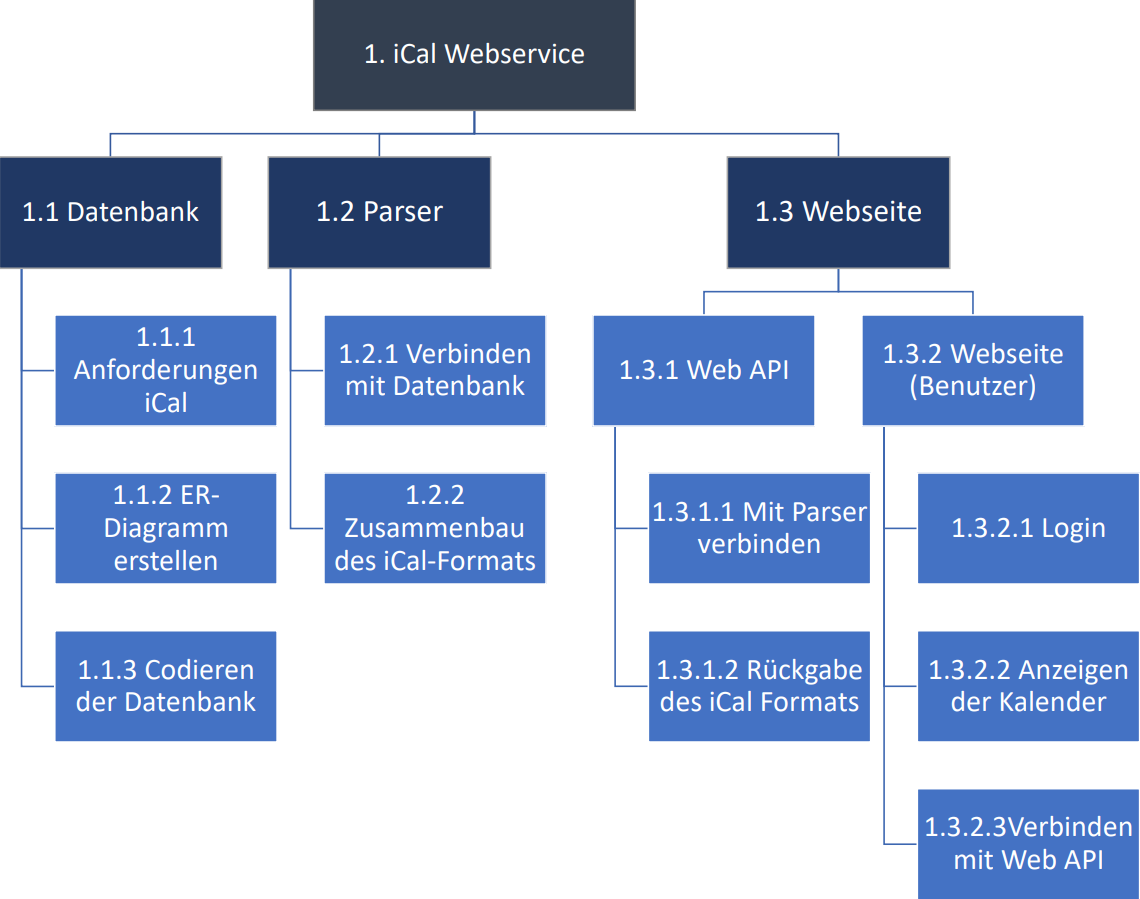
\includegraphics[width=\textwidth]{ProjektmanagementUndOrganisation_Projektstrukturplan.png}
    \caption{Projektstrukturplan}
    \label{fig:projektStrukturplan}
\end{figure}

\subsection{VMI-Matrix}
\label{sec:VMI-Matrix}
Eine VMI-Matrix ist ein wichtiges Projektmanagementinstrument, welches dazu dient, Verantwortlichkeiten innerhalb eines Projektes darzustellen. In einer VMI-Matrix ist für jedes Arbeitspaket genau erkennbar, wer in welcher Art damit zu tun hat. Es gibt drei Arten von Verantwortlichkeiten: \\ \\
\textbf{V} ... Diese Person trägt Verantwortung für das Erreichen des Ziels und Einhaltung der Ressourcenvorgaben.\\ \\
\textbf{M} ... Diese Person ist unterstützend tätig.\\ \\
\textbf{I} ... Diese Person wird über Ereignisse betreffend dieses Arbeitspaketes informiert. Er oder sie muss nicht aktiv daran arbeiten informiert zu werden, sondern die Verantwortlichen müssen den zu Informierenden selbstständig informieren.\\ \\
Wie eine VMI-Matrix aussieht ist in Abbildung \ref{fig:vmi-Matrix} zu sehen. Ein vollständiger Projektstrukturplan erleichtert die Erstellung einer VMI-Matrix, da die Arbeitspakete des Projektstrukturplans sind abwandelbar und können somit in eine VMI-Matrix eingetragen werden können. Eine Erklärung des Projektstrukturplans ist im Kapitel \ref{ref:Projektstrukturplan}.\\vgl. 
\textcite{VMI-Matrix}\\

\begin{figure}[H]
	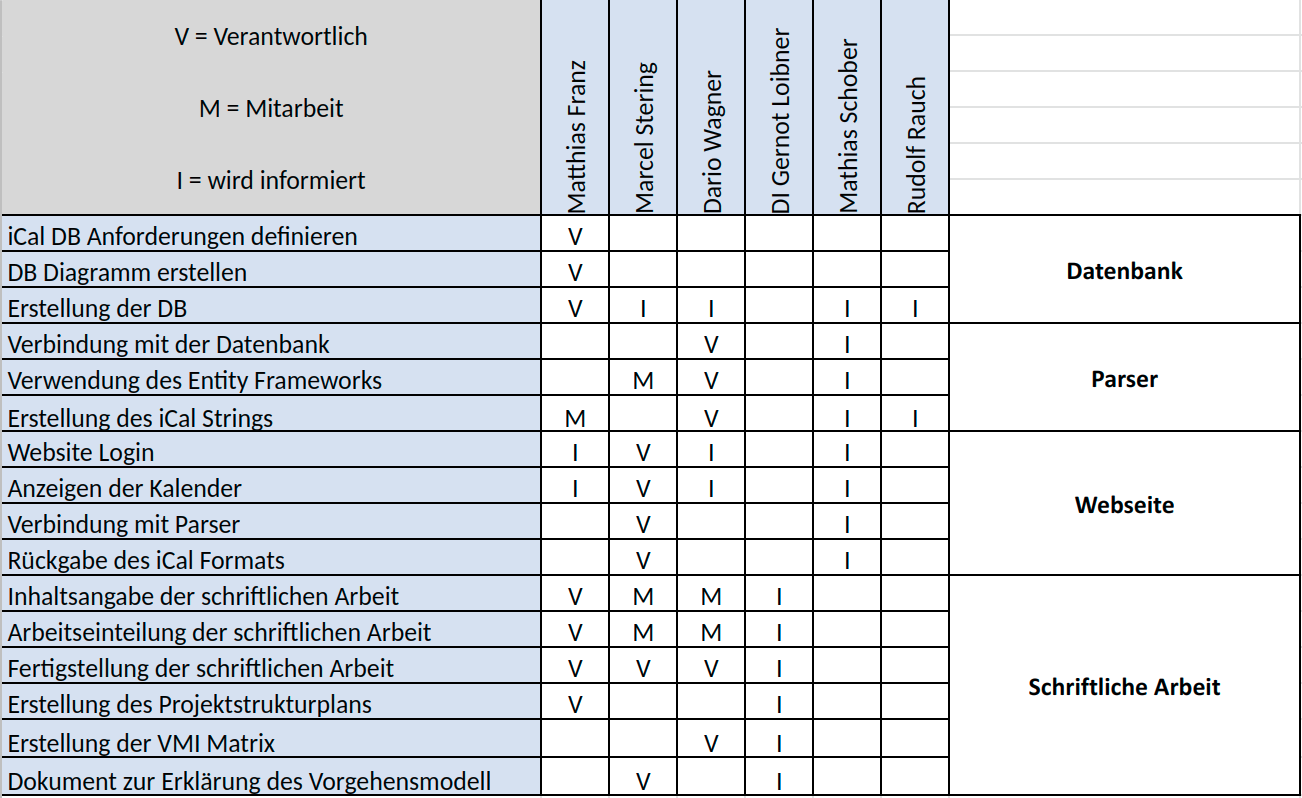
\includegraphics[width=\textwidth]{ProjektmanagementUndOrganisation_VMI-Matrix.png}
    \caption{VMI-Matrix}
    \label{fig:vmi-Matrix}
\end{figure}


\pagebreak	
		
